\chapter{Results} \label{chap:Results}

%The results chapter should simply present the results of applying the methods presented in the method chapter without further ado. This chapter will typically contain many graphs, tables, etc. Sometimes it is natural to discuss the results as they are presented, combining them into a `Results and Discussion' chapter, but more often they are kept separate.\\ 

The following sections presents the results for each attack type, with subsections for the detection threshold levels selected, as defined in section \ref{sec:ExpDef} \\ 

Comments on the results are deferred to chapter \ref{chap:Discussions}
\newpage
\section{Ascending delay function}
\begin{figure}[hb]
 %   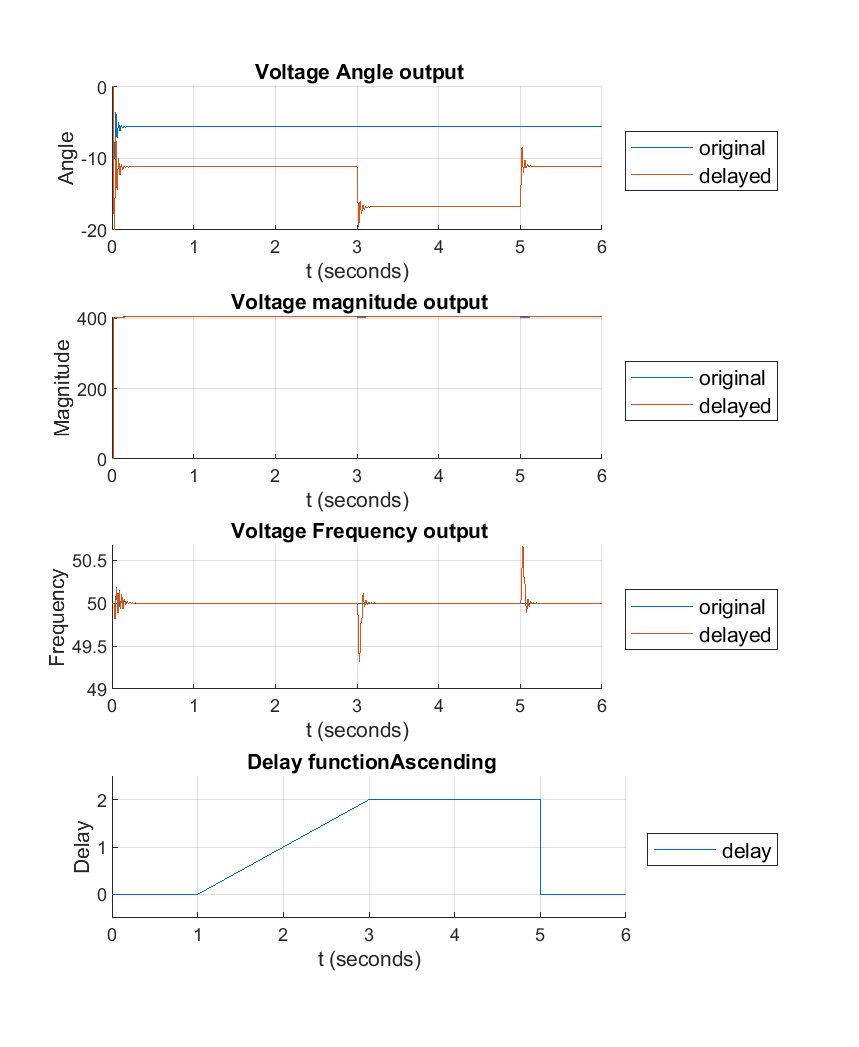
\includegraphics[trim=2 10 14 4, clip]{figures/v_AllFig-DelayOf_2-Ascending.png}    
    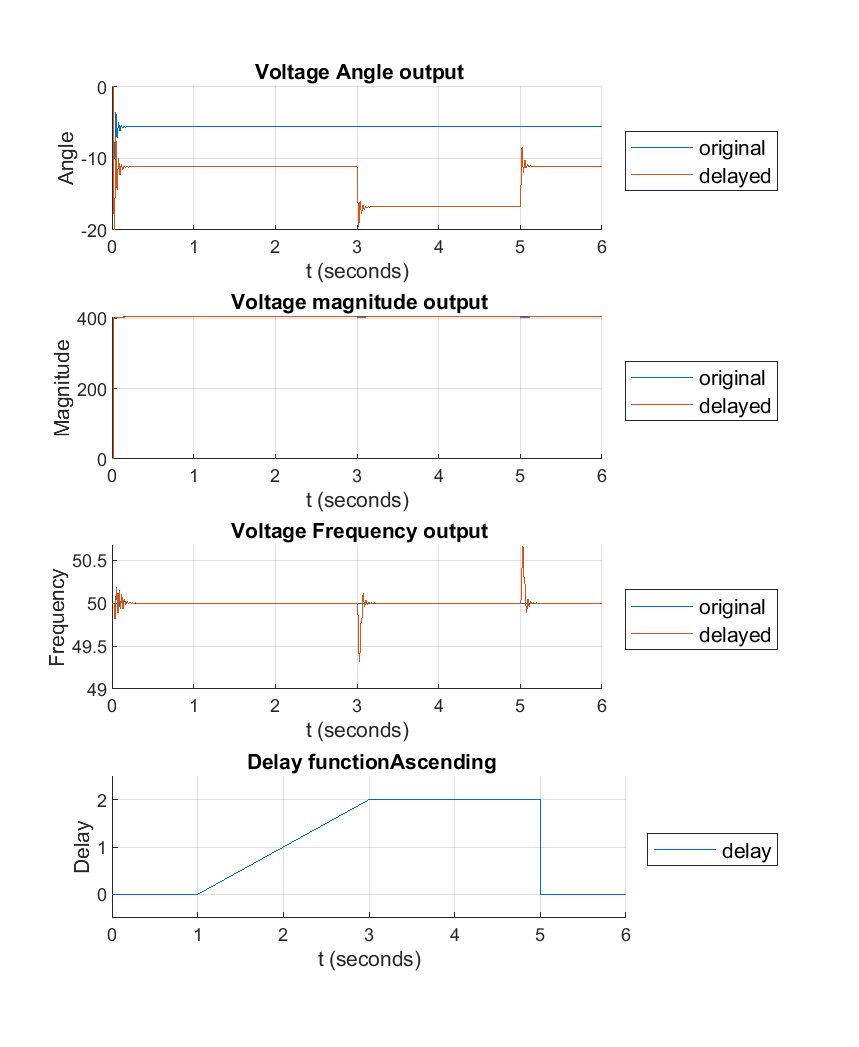
\includegraphics[width=0.95\textwidth]{figures/v_AllFig-DelayOf_2-Ascending.png}    
    \caption{Ascending delay combined output}
    \label{fig:simPMU-allfig}
\end{figure}


     \begin{figure}
        \caption{Component-wise output}
 
    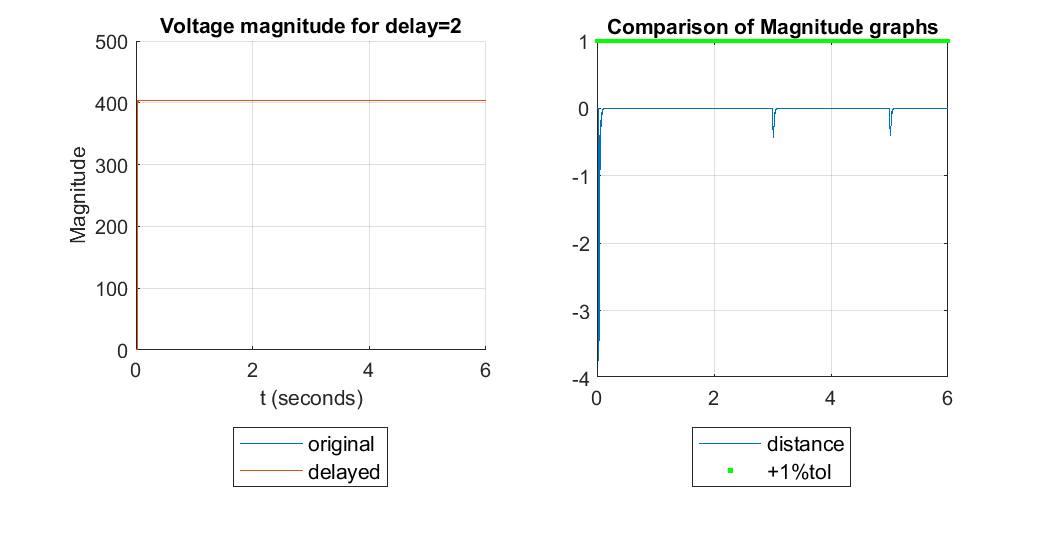
\includegraphics[width=0.95\textwidth]{figures/v_MagFig-DelayOf_2-Ascending.png}    
         %\caption{magnitude Output}
         \label{fig:AscMag}
   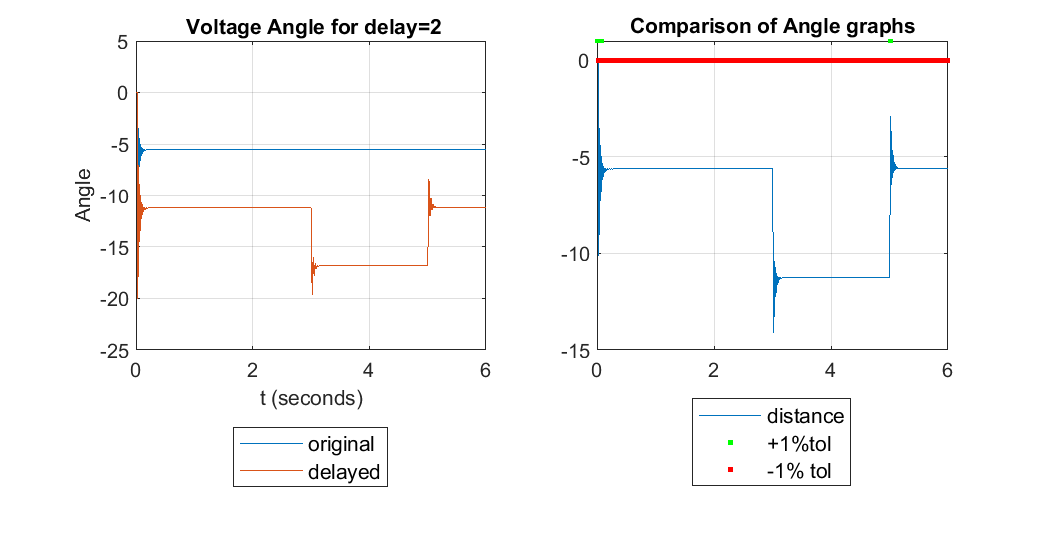
\includegraphics[width=0.95\textwidth]{figures/v_AngFig-DelayOf_2-Ascending.png}    
          %\caption{Angle Output}
         \label{fig:AscAng}
   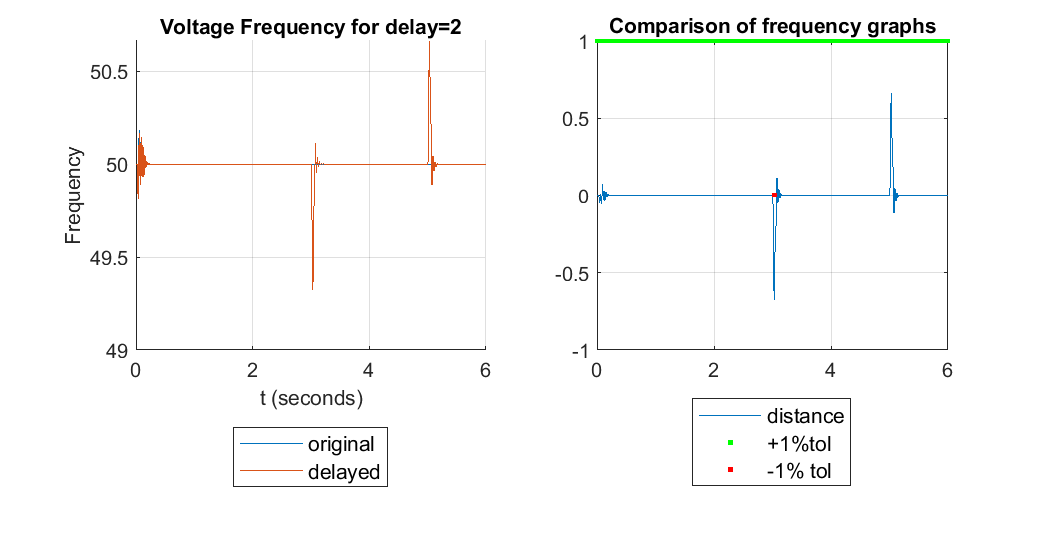
\includegraphics[width=0.95\textwidth]{figures/v_FreqFig-DelayOf_2-Ascending.png}    
         %\caption{frequency Output}
         \label{fig:AscFreq}
 
\end{figure}






\newpage
\section{Ascending delay function: Delay of 6}
\begin{figure}[hb]
 %   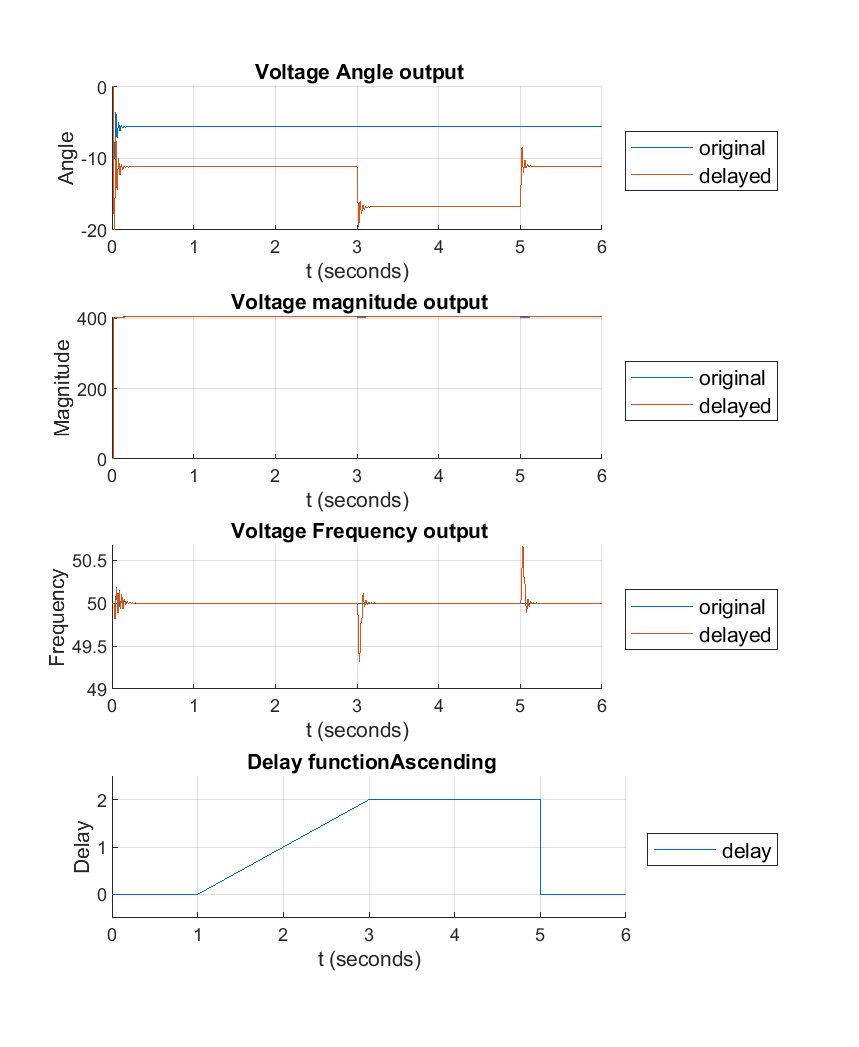
\includegraphics[trim=2 10 14 4, clip]{figures/v_AllFig-DelayOf_2-Ascending.png}    
    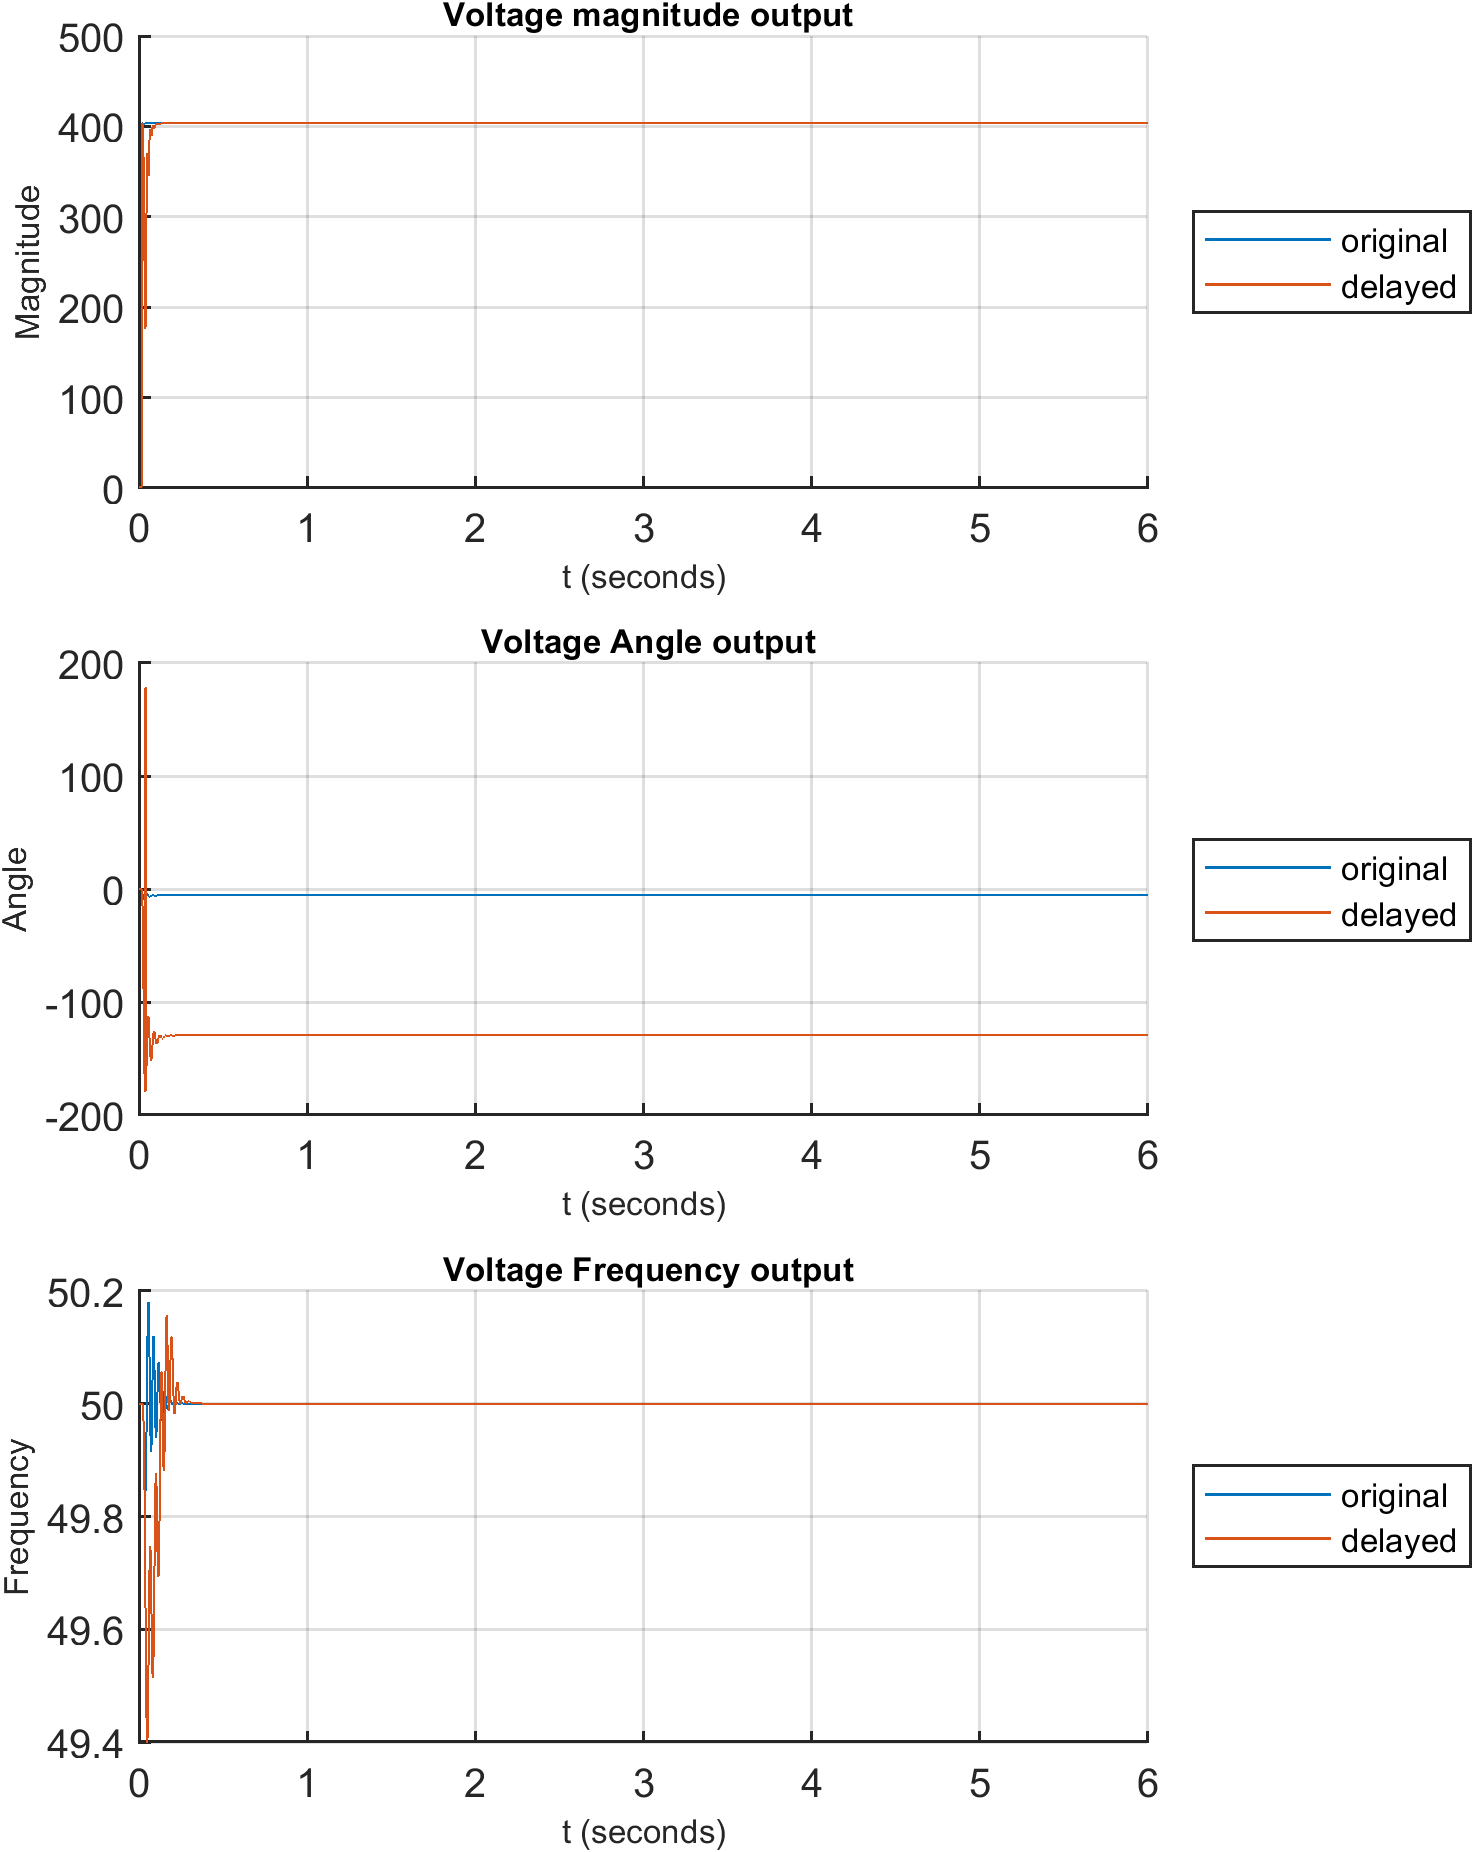
\includegraphics[width=0.95\textwidth]{\locateResults/AllFig.png}    
    \caption{Ascending delay combined output}
    \label{fig:PMUsim-Asc6-allfig}
\end{figure}


     \begin{figure}
        \caption{Magnitude component output}
 
    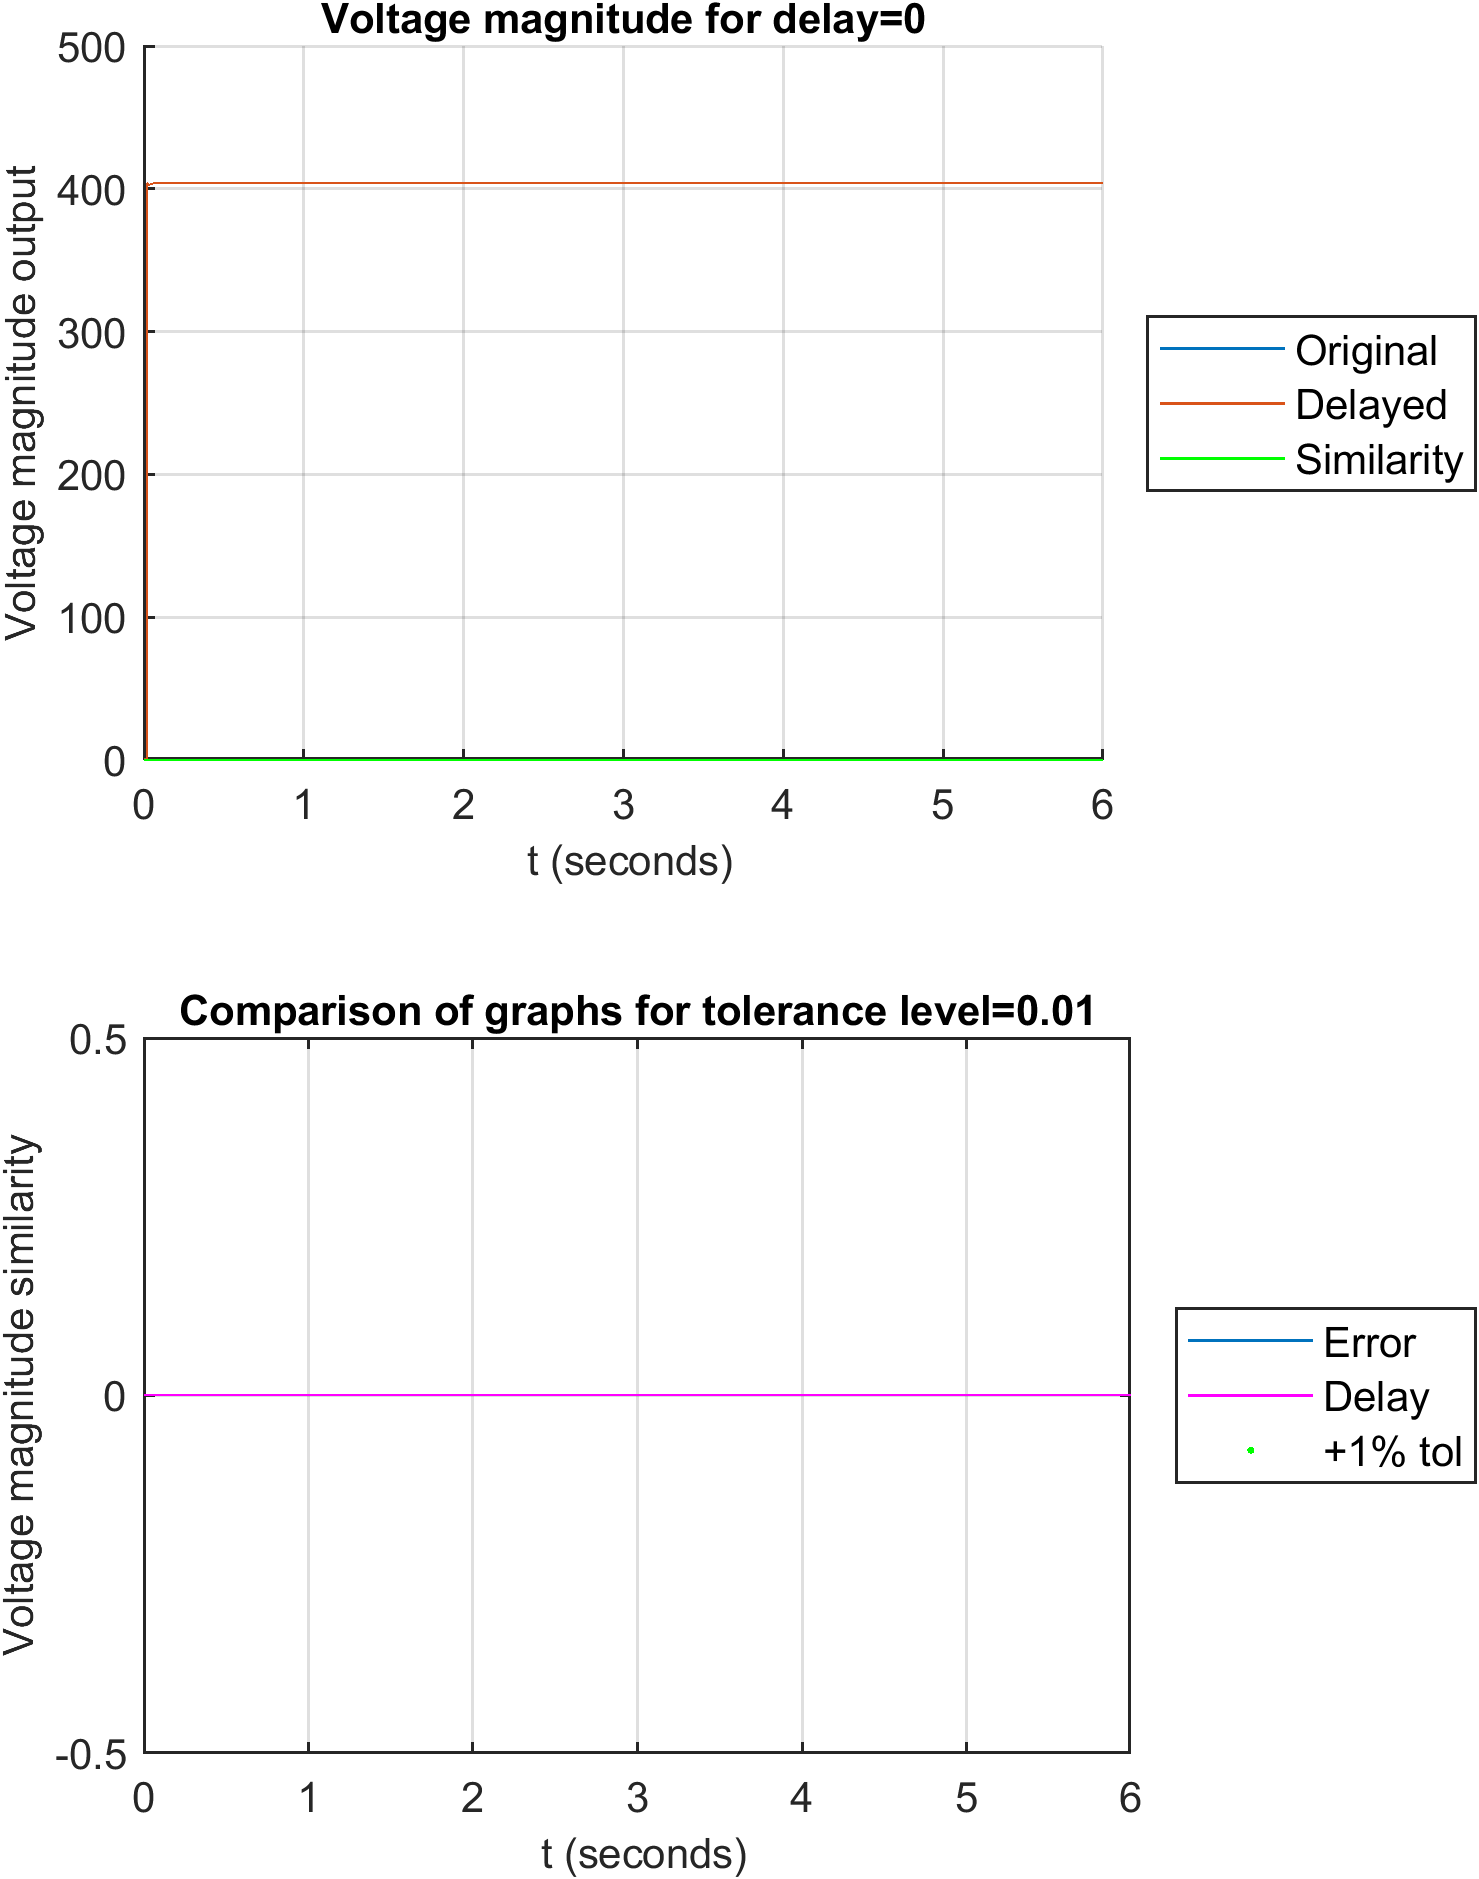
\includegraphics[width=1.25\textwidth]{\locateResults/Magnitude.png}    
         %\caption{magnitude Output}
         \label{fig:PMUsim-Asc6Mag}
 
\end{figure}

     \begin{figure}
        \caption{Angle component output}
 
   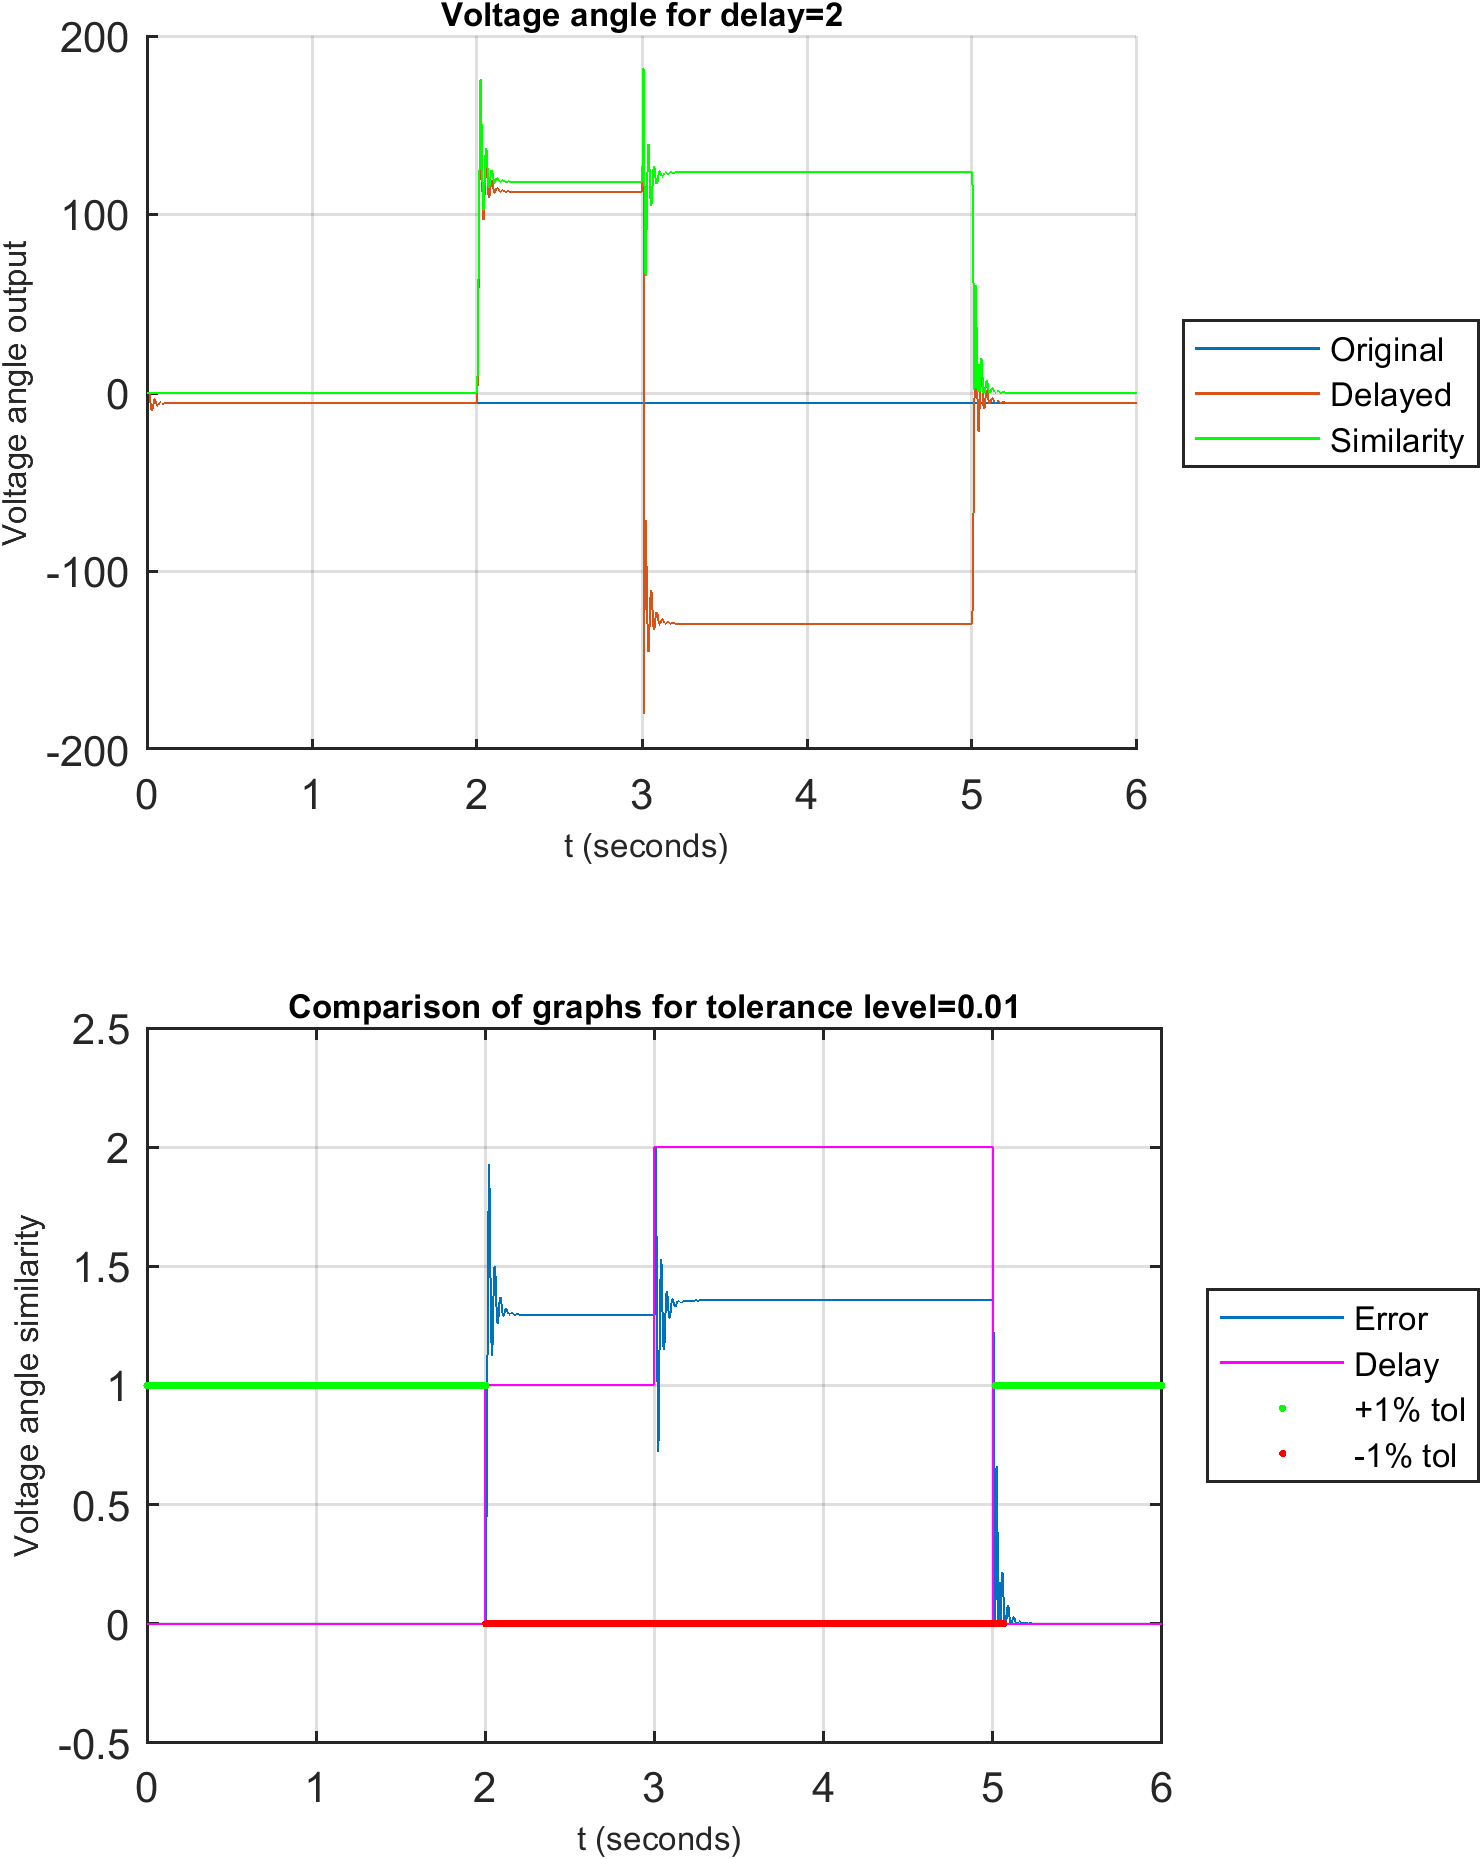
\includegraphics[width=1.25\textwidth]{\locateResults/Angle.png}    
          %\caption{Angle Output}
         \label{fig:PMUsim-Asc6Ang}
 
\end{figure}

     \begin{figure}
        \caption{Frequency component output}
 
   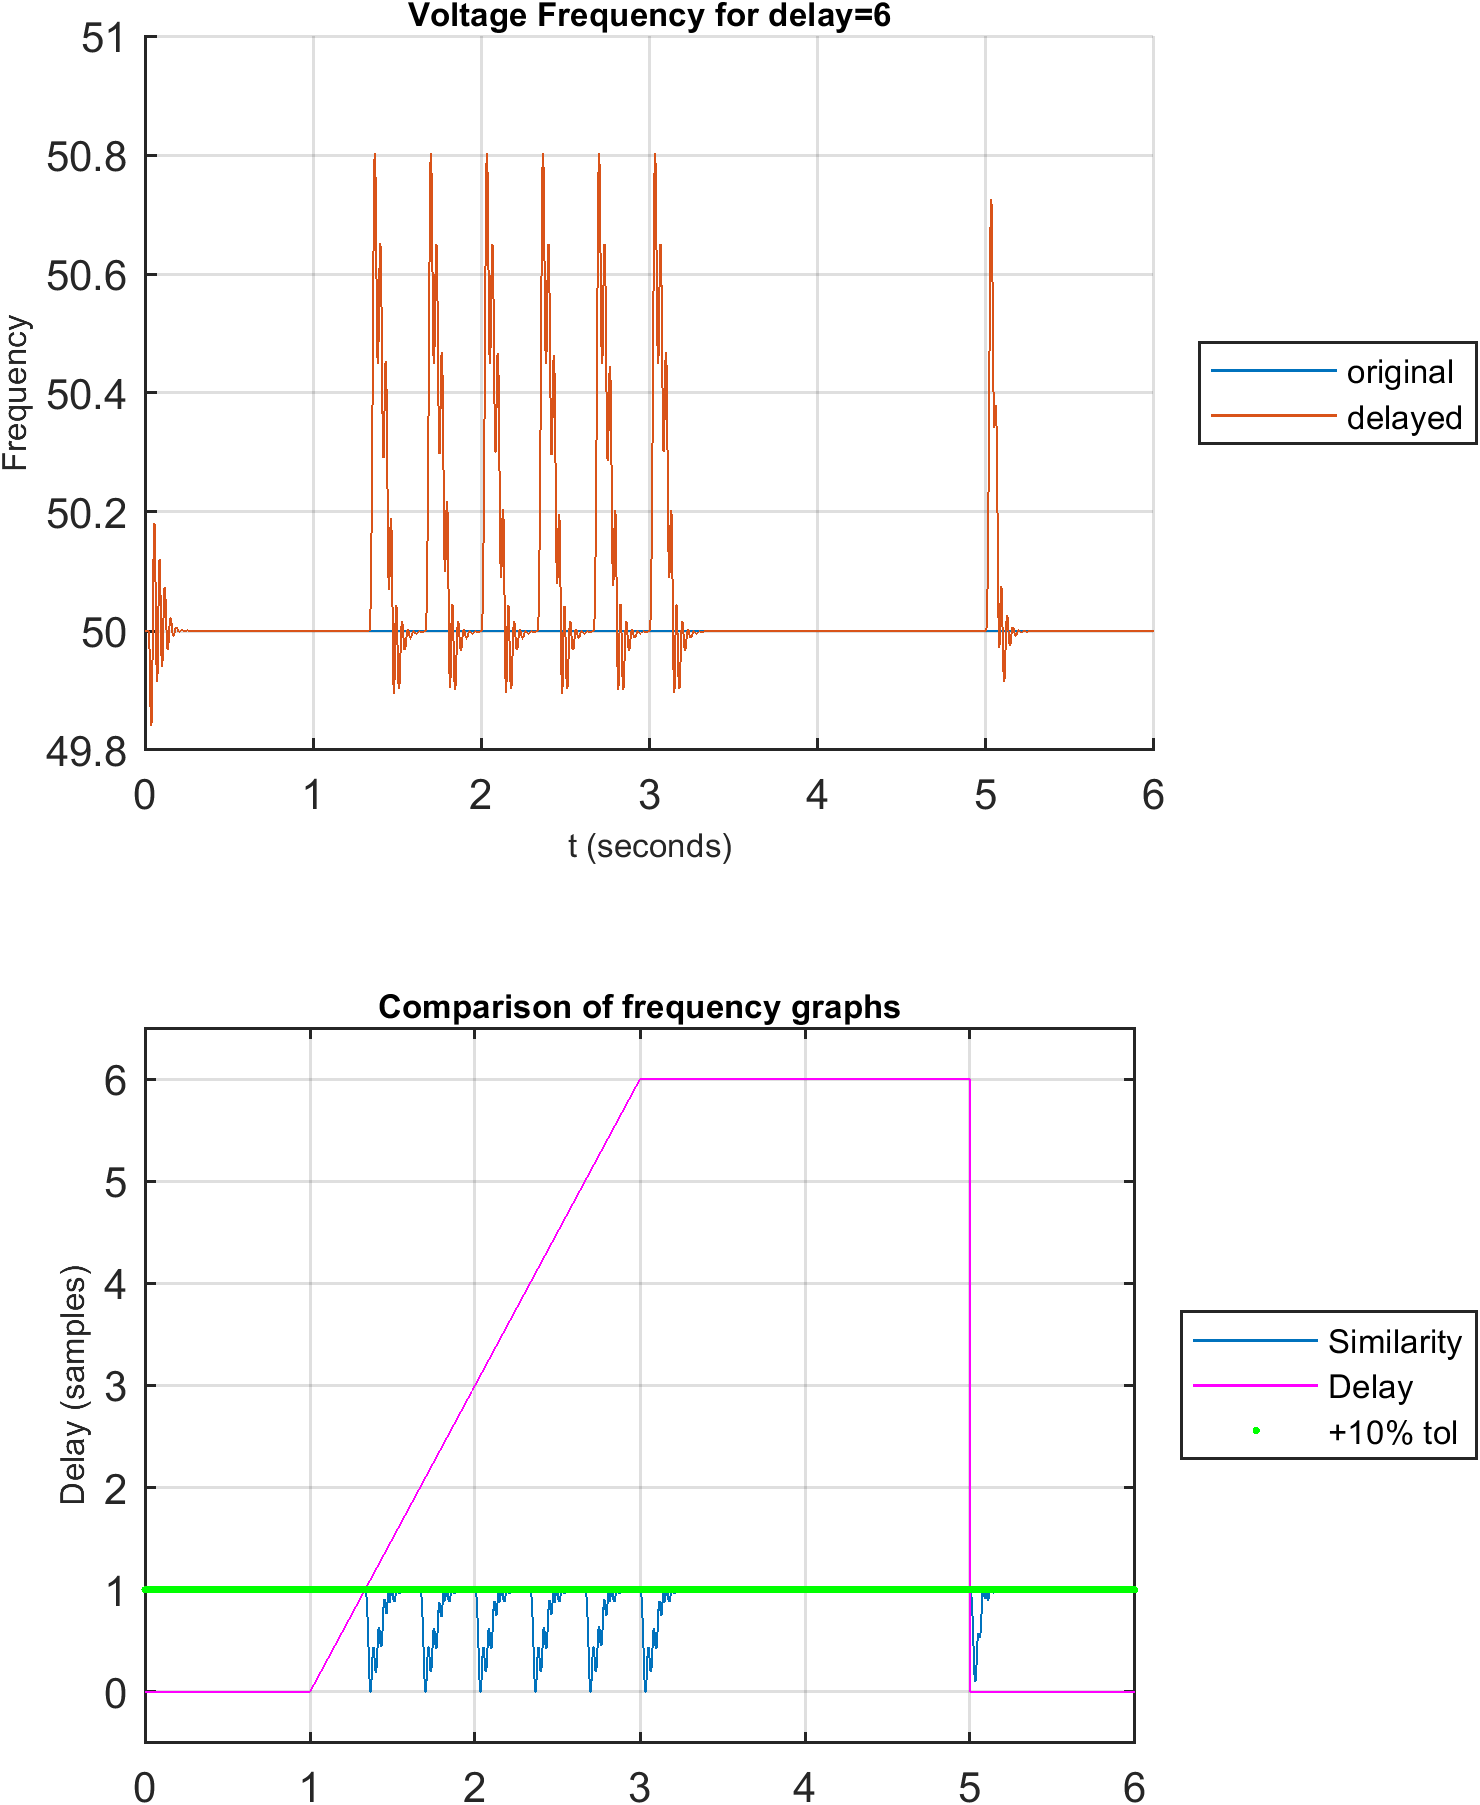
\includegraphics[width=1.25\textwidth]{\locateResults/Frequency.png}    
         %\caption{frequency Output}
         \label{fig:PMUsim-Asc6Freq}
 
\end{figure}











%\section{off, on, off: abrupt}
%\subsection{Findings for a detection threshold level of 0.01}
%\subsection{Findings for a detection threshold level of 0.05}
%\subsection{Findings for a detection threshold level of 0.10}

%\section{increasing, on , decreasing: small steps}
%\subsection{Findings for a detection threshold level of 0.01}
%\subsection{Findings for a detection threshold level of 0.05}
%\subsection{Findings for a detection threshold level of 0.10}

%\section{increasing and continuous}
%\subsection{Findings for a detection threshold level of 0.01}
%\subsection{Findings for a detection threshold level of 0.05}
%\subsection{Findings for a detection threshold level of 0.10}

%\subsection{Findings for a detection threshold level of 0.01}
%\subsection{Findings for a detection threshold level of 0.05}
%\subsection{Findings for a detection threshold level of 0.10}
%\section{Findings for delay level 0.11}
%\section{Findings for delay level 0.12}
%\section{Findings for delay level 0.13}
%\section{Findings for delay level 0.14}
%\section{Findings for delay level 0.15}


